\documentclass{article}

\usepackage{amsmath} % math stuff
\usepackage{amssymb} % math stuff
\usepackage{array} % equations and stuff
\usepackage{bm} % bold math
%\usepackage{booktabs} % extra table rule options
%\usepackage{caption} % suppressed table numbering; incompatible with revtex, and longtable, I think
\usepackage{comment} % comment environment
%\usepackage{enumitem} % customization of enumeration, itemize, and description
\usepackage[T1]{fontenc} % font encoding for special characters, must also use scalable font package
\usepackage[margin=0.8in]{geometry} % paper sizes and margins (but be careful not to mess up pre-defined pages)
\usepackage{graphicx} % for graphics
%\usepackage{helvet} % default font is the helvetica postscript font
\usepackage[utf8]{inputenc} % special characters in tex input
\usepackage{layouts} % print units like widths
\usepackage{lipsum} % lorem ipsum filler text
\usepackage{lmodern} % scalable font?
\usepackage{longtable} % multi-page tables
\usepackage{makecell} % specify line-breaks in table cells
\usepackage{mathrsfs} % math script font
\usepackage{mhchem} % easier chemical formula
\usepackage{microtype} % allows disabling of ligatures
\usepackage{multicol} % multicolumns
%\usepackage{newcent} % new century schoolbook font
\usepackage{nicefrac}
\usepackage{numprint} % print and format (large) numbers
\usepackage{parskip} % removes paragraph indentation, and adjusts paragraph skip, as well as list items
\usepackage{pdfpages} % add pdf files as pages
%\usepackage{setspace} % adjust text spacing and indents
\usepackage{siunitx} % decimal alignment, and degree symbol
\usepackage{subfigure} % divided figures
%\usepackage{tabu} % extra table options
\usepackage{textcomp} % symbols
\usepackage{threeparttablex} % better footnotes with longtable
\usepackage{titling} % title placement
\usepackage{ulem} % strikethrough text
\usepackage{upgreek} % upright Greek letters
%\usepackage{url} % superceded by hyperref
\usepackage{verbatim} % verbatim environment
\usepackage{xcolor} % colors and color boxes
\usepackage{xspace} % commands that don't eat up white space
\usepackage{hyperref} % links and page setup; should always come last

\hypersetup{
 bookmarks=true,
 colorlinks=true,
 citecolor=blue,
 linkcolor=blue,
 urlcolor=blue,
 pdfstartview={XYZ null null 1.0} % default open view is 100%
}

\DisableLigatures[f,t]{encoding = T1} % disable ff, fi, fl, tt ligatures; without options, it also disables -- = endash
\renewcommand{\arraystretch}{1.0} % extra vertical (and horizontal?) space in tables

% define centered, left- and right-aligned columns with specified widths
\newcommand{\PreserveBackslash}[1]{\let\temp=\\#1\let\\=\temp}
\newcolumntype{C}[1]{>{\PreserveBackslash\centering}p{#1}}
\newcolumntype{L}[1]{>{\PreserveBackslash\raggedright}p{#1}}
\newcolumntype{R}[1]{>{\PreserveBackslash\raggedleft}p{#1}}

\begin{document}

\pagestyle{empty} % don't number pages

% custom title
\begin{center}
{\LARGE Classic Riddler}

\vspace{0.15in}

{\Large 4 March 2022}
\end{center}


\section*{Riddle:}

Two ants named Geo and Desik are racing along the surface of a cone.
The circular base of the cone has a radius of 2 meters and a slant height of 4 meters.
Geo and Desik both start the race on the base, a distance of 1 meter away from its center.

The race's finish is halfway up the cone, 90 degrees around the cone's central axis from the start, as shown in the following diagram:

\vspace{0.1in}
\begin{center}
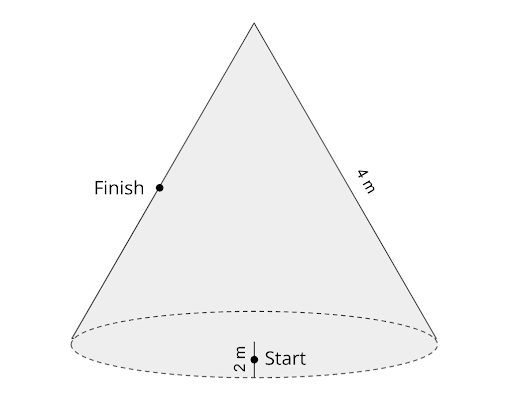
\includegraphics[width=3in]{cone.png}
\end{center}
\vspace{0.1in}

Geo and Desik both want your help in strategizing for the race.
What is the length of the shortest path from the start to the finish?


\section*{Solution:}

Because the base is a circle with radius 2, the edge of the cone has a circumference of $4\pi$.
The top surface of the cone could be unfolded into a circular segment with radius 4.
This segment must also have an arc length of $4\pi$.
This is half the circumference of a circle of radius 4 ($8\pi$), so the segment must be a semicircle.

I set up the diagrams as shown on the final page.
For the coordinate system of the base circle, I define the start point $x_{1}$ to be along the x-axis, and the finish point to be above the y-axis.
Then the ideal path will exit the base at $x_{2}$, at some angle $\theta$ relative to the x-axis.
The two points are then

\begin{align*}
x_{1} &= (1,0) \\
x_{2} &= (2\cos\theta,2\sin\theta)
\end{align*}

and the path length $L_{1}$ between them is

\[
L_{1} = \sqrt{(1-2\cos\theta)^2+(2\sin\theta)^2}
\]

For coordinate system of the semicircle, I keep the start point below the x-axis.
Because the full circumference of the cone is compressed by half, the finish point is located at a 45\textdegree\ angle relative to the x-axis.
The entry point $x_{3}$ is at some angle $\phi$, and $x_{4}$ is the finish point.
These two points are

\begin{align*}
x_{3} &= (4\cos\phi,4\sin\phi) \\
x_{4} &= (\sqrt{2},\sqrt{2})
\end{align*}

and the path length $L_{2}$ between them is

\[
L_{2} = \sqrt{(\sqrt{2}-4\cos\phi)^2+(\sqrt{2}-4\sin\phi)^2}
\]

Because of the angular compression between the two coordinate systems, $\theta=2\phi$.
I use this substitution and some trigonometric identities to get the total path length $L=L_{1}+L_{2}$

\[
L = \sqrt{5-4(\cos^{2}\phi-\sin^{2}\phi)} + \sqrt{20-8\sqrt{2}(\cos\phi+\sin\phi)}
\]

Plugging in this equation into Wolfram Alpha gives a minimum at $\phi\approx0.2618$ with a total path length of (approximately) \fcolorbox{red}{white}{\textbf{3.718~m}}\,.

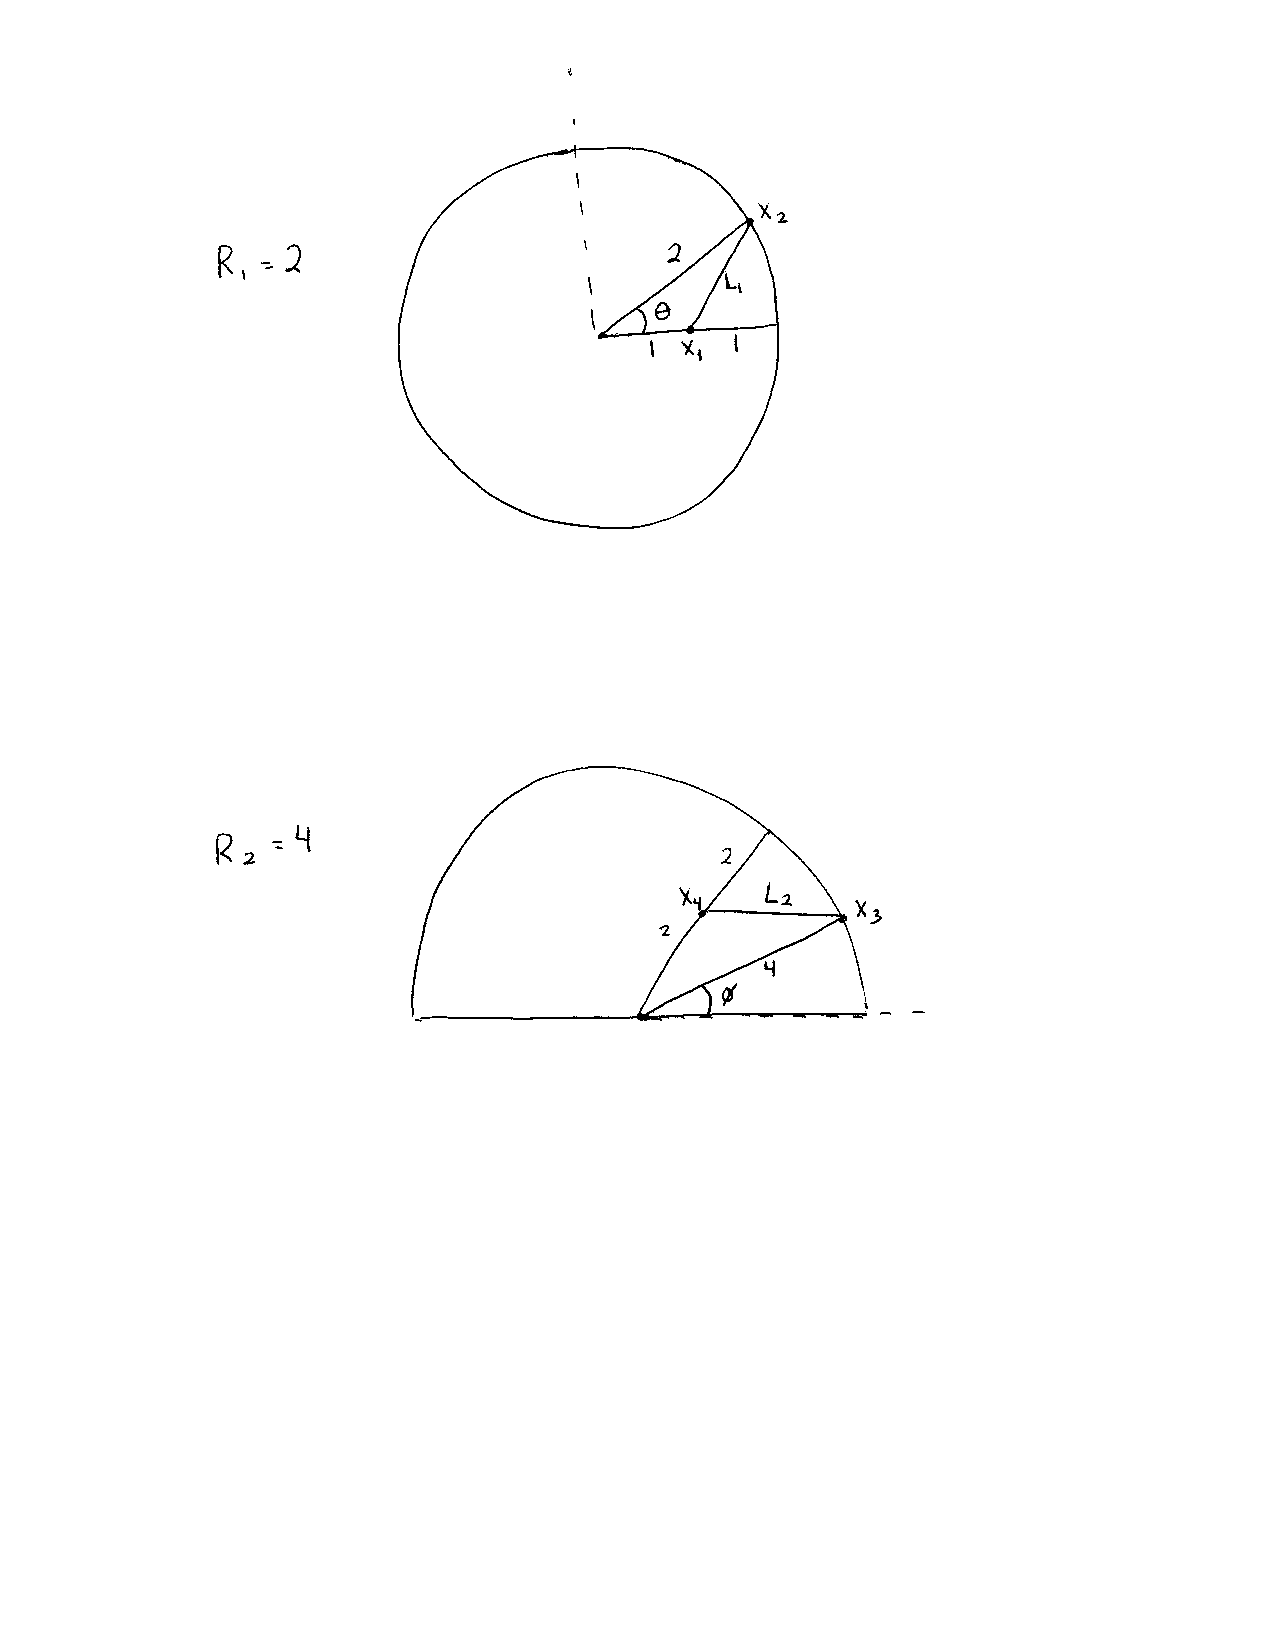
\includepdf{cone_diagram.pdf}


\end{document}